\chapter{TODO: Kapitola o zmensovani a rozoberani "specialnych" pripadov}

Časová zložitosť algoritmu Junosza-Szaniawski je principiálne veľká na grafoch, v ktorých
existuje veľa rôznych čiastočných $L(2,1)$ ofarbení. Ako sme videli v predošlej kapitole,
spomedzi súvislých grafov majú najviac čiastočných ofarbení, resp. vlastných párov, stromy.
Na dostatočne jednoduchých triedach grafov však existujú polynomiálne algoritmy, ktoré
riešia problém $L(2,1)$-farbenia.

Intuitívne platí, že pri jednoduchých grafoch vieme problém rozdeliť na viacero menších,
menšie problémy vyriešiť nezávisle a nakoniec ich riešenia pospájať. V tejto kapitole
sa pozrieme na spôsob, akým vieme túto intuíciu aplikovať.

Aj keď v práci rozoberáme problém $L(2,1)$-farbenia, postupy z tejto kapitoly sa principiálne
dajú aplikovať aj na všeobecnejšie $L(p,q)$-farbenia.

\section{Teoretické základy rozdelenia problému}

Ako sa ďalej v práci ukáže, aby sme vedeli problém dobre rozdeliť, potrebujeme riešiť
o trochu všeobecnejší problém: Každému vrcholu grafu pridáme obmedzenie na hodnoty,
ktorými môže byť ofarbený.

FIXME: Zmenit problem a prepisat vsade. Nechceme zoznam povolenych hodnot, chceme mat nejake
ciastocne ofarbenie a doplnit ho. Toto potom vie J-S riesit v case $a^n$ bez ohladu na ostatne
veci.

\begin{defn}
    Rozhodovací problém \emph{doplnenia $L(2,1)$-farbenia} definujeme nasledovne: Inštanciou je
    graf $G$, prirodzené číslo $k$ a čiastočné $L(2,1)$-farbenie $f$ množiny $S \subseteq V(G)$
    v grafe $G$, kde rozsah $f$ je nanajvýš $k$.

    Inštancia je riešiteľná práve vtedy, keď existuje $L(2,1)$ farbenie
    $f'$ grafu $G$ s rozsahom $k$, pre ktoré platí: $\forall v \in S: f'(v) = f(v)$.
\end{defn}

Ľubovoľné riešenie problému doplnenia $L(2,1)$-farbenia vieme prerobiť na riešenie
problému $L(2,1)$-farbenia, ak za čiastočné farbenie $f$ vezmeme prázdne farbenie.
Mnohé riešenia problému $L(2,1)$-farbenia sa dajú prerobiť na riešenia problému
doplnenia $L(2,1)$-farbenia bez výrazného zhoršenia časovej zložitosti.
Ukážeme si to na príklade algoritmu Junosza-Szaniawski.

Najprv si pripomenieme, ako funguje algoritmus Junosza-Szaniawski.
Tento algoritmus postupne počíta tabuľky $T_0, T_1, \ldots T_{2n}$.
Tabuľka $T_i$ obsahuje reprezentáciu všetkých čiastočných $L(2,1)$-farbení grafu s rozsahom $i$. Pre každé
čiastočné farbenie v tabuľke $T_i$ vieme povedať zoznam vrcholov, ktoré používajú farbu $i$.

Úprava algoritmu teda bude spočívať v tom, že po vypočítaní tabuľky $T_i$ z nej odstránime
všetky čiastočné farbenia, ktoré nejakému vrcholu $v \in S$ priradili inú hodnotu, ako $f(v)$.

Pozor si však treba dať na počet tabuliek, ktoré potrebujeme vypočítať. Keďže niektoré vrcholy
majú predpísanú farbu, nemusí existovať triviálne farbenie s rozsahom $2n$. Ďalej však dokážeme,
že všetky vrcholy mimo množiny $S$ vieme triviálne ofarbiť farbami veľkosti nanajvýš $3n$. Keďže
časová zložitosť počítania tabuľku $T_i$ z tabuľky $T_{i-1}$ je $O^*(2.6488^n)$ a tento výpočet
spravíme najviac $(3n)$-krát, časová zložitosť tohto algoritmu bude $O^*(2.6488^n)$.

\begin{lema}
    Nech $f$ je čiastočné $L(2,1)$-farbenie množiny $S$ v grafe $G$. Potom existuje
    $L(2,1)$-farbenie $f'$ grafu $G$, ktoré dopĺňa $f$ a pre ktoré platí $\ \forall v \in V(G) - S: f(v) < 3n$.
\end{lema}
\begin{proof}
    Základná myšlienka dôkazu je nasledovná. Vezmeme množinu farieb, ktoré sú priradené vrcholom v $S$
    a označíme ju $F$. Ak nájdeme množinu farieb $F'$, ktorá má veľkosť (aspoň) $|V(G) - S|$,
    každá dvojica farieb v nej má rozdiel aspoň $2$ a každá dvojica farieb $(c_1, c_2) \in F \times F'$ má
    rozdiel aspoň $2$, tak neofarbeným vrcholom môžeme ľubovoľne priradiť farby z $F'$ a dostneme
    $L(2,1)$-farbenie.

    V každej trojici čísel $(3x, 3x + 1, 3x+2)$, kde $0 \leq x < n$, buď existuje vrchol
    v množine $S$, ktorý má priradenú jednu z týchto farieb, alebo sa farba $3x + 1$ môže nachádzať v
    množine $F'$. Ak má množina $S$ presne $m$ vrcholov, nájdeme takto $n - m$ farieb, ktoré
    môžeme priradiť vrcholom vo $V(G) - S$.
\end{proof}
\begin{dosl}
    Nech $(G, k, f)$ je inštancia problému doplnenia $L(2,1)$-farbenia. Ak $k \ge 3n$, tak
    je inštancia riešiteľná.
\end{dosl}

\subsection{Rozdelenie na hranových separátoroch}

Prvý typ ``jednoduchosti'' grafu, ktorú vieme využiť pri hľadaní rýchlejšieho algoritmu,
zodpovedá hranovej súvislosti grafu. Vezmime si nejaký hranový separátor $S_E$ grafu $G$. 
Všetkým vrcholom, ktoré sú incidentné s niektorou hranou separátora, zafixujeme nejaké farby.
Ďalej si vezmime komponenty súvislosti grafu $G - S_E$.

Ak v každom komponente súvislosti nájdeme (nezávisle) nejaké $L(2,1)$-farbenie
konzistentné s ohodnotením separátora, spojením farbení pre každý podgraf dostaneme
$L(2,1)$-farbenie celého grafu $G$. Toto tvrdenie si formálne zhrnieme v nasledujúcej leme.

\begin{lema}
\label{hrsep-lema}
    Nech $S_E \subseteq E(G)$ je hranový separátor grafu $G$,
    nech $S_V \subseteq V(G)$ je množina všetkých vrcholov, ktoré sú incidentné s niektorou hranou
    v $S_E$, nech $G_1, G_2, \cdots G_k$ sú komponenty súvislosti grafu $G - S_E$.

    Nech $f_S: S_V \to \mathbb{N}$ je čiastočné $L(2,1)$-farbenie množiny $S_V$ v grafe $G$,
    nech $f_1, f_2, \ldots, f_k$ sú čiastočné $L(2,1)$-farbenia množín $V(G_1) \cup S_V,\ 
    V(G_2) \cup S_V,\  \ldots, V(G_k) \cup S_V$ v grafe $G$ a nech platí

    $$ \forall i \in {1 \ldots k},\  \forall v \in S_V: f_i(v) = f_S(v) .$$

    Potom zobrazenie $\omega: V(G) \to \mathbb{N}$ definované nasledovne:

    \[ \omega(v) =
    \begin{cases}
        f_S(v), & v \in S_V \\
        f_i(v), & v \in V(G_i) - S_V
    \end{cases}
    \]

    tvorí $L(2,1)$-farbenie grafu $G$.

\end{lema}

\begin{proof}
    Zobrazenie $\omega$ je dobre definované, lebo každý vrchol patrí do práve jedného komponentu grafu
    $G - S_E$, zároveň každému vrcholu v $G$ priradí hodnotu. Potrebujeme teda overiť podmienky $L(2,1)$-farbenia
    pre každú dvojicu vrcholov $u, v \in V(G)$. Ďalej rozoberieme niekoľko prípadov podľa príslušnosti $u, v$:

    \begin{description}
        \item[Oba vrcholy patria do množiny $S_V$:] Z definície $\omega$ platí $\omega(u) = f_S(u), \omega(v) = f_S(v)$.
        Keďže $f_S$ je čiastočné $L(2,1)$-farbenie množiny $S_V$, vrcholy $u, v$ musia spĺňať podmienky $L(2,1)$-farbenia.

        \item[Vrchol $u$ patrí do $S_V$, vrchol $v$ do $V(G_i) - S_V$ pre niektoré $i$:] Z definície $\omega$ platí
        $\omega(u) = f_S(u) = f_i(u)$ a $\omega(v) = f_i(v)$. Keďže $f_i$ je čiastočné $L(2, 1)$-farbenie, vrcholy
        $u, v$ musia spĺňať podmienky $L(2,1)$-farbenia.
        
        \item[Oba vrcholy patria do toho istého komponentu $G_i$:] Z definície
        $\omega$ platí $\omega(u) = f_i(u), \omega(v) = f_i(v)$. Keďže $f_i$ je čiastočné $L(2,1)$-farbenie, vrcholy
        $u, v$ musia spĺňať podmienky $L(2,1)$-farbenia.

        \item[Vrchol $u$ patrí do komponentu $G_i$, vrchol $v$ do komponentu $G_j$, $i \neq j$:] Keďže vrcholy patria
        do rôznych komponentov grafu $G - S_E$, každá cesta medzi $u, v$ obsahuje aspoň jednu hranu z $S_E$. Špeciálne
        to platí pre každú najkratšiu cestu medzi $u$ a $v$. Keďže $u, v \notin S_V$, každá najkratšia cesta medzi $u$
        a $v$ musí pozostávať z neprázdnej cesty z $u$ do niektorého vrchola v $S_V$, hrany v $S_E$ a z neprázdnej
        cesty z vrchola v $S_V$ do vrchola $v$. To znamená, že vrcholy $u$ a $v$ sú vzdialené aspoň $3$, teda spĺňajú
        podmienky $L(2,1)$-farbenia.
    \end{description}

    Každá dvojica vrcholov spĺňa obmedzenia $L(2,1)$-farbenia, a preto $\omega$ je $L(2,1)$-farbením grafu $G$. \qedhere

\end{proof}

\begin{dosl}
    Nech $e \in E(G)$ je most grafu $G$, nech $u, v$ sú vrcholy hrany $e$, nech graf $G - \{e\}$ pozostáva z dvoch
    komponentov $G_1$ a $G_2$ veľkosti aspoň $2$. Potom je graf $G$ $k$-$L(2,1)$-zafarbiteľný práve vtedy, ak
    existujú hodnoty $a, b$ také, že $0 \leq a, b \leq k, \left| a - b \right| \ge 2$ a existujú $k$-$L(2,1)$-farbenia $f_1, f_2$ grafov
    $G_1 \cup \{v, u, e\}$ a $G_2 \cup \{v, u, e\}$, pre ktoré platí $f_1(u) = f_2(u) = a \wedge f_1(v) = f_2(v) = b$.
\end{dosl}

\begin{proof}
    $\boxed{\Rightarrow}$
        Ak je graf $G$ $k$-$L(2,1)$-zafarbiteľný, existuje jeho $k$-$L(2,1)$-farbenie $f$. Zobrazenia $f_1, f_2$ môžeme
        definovať ako zúženie zobrazenia $f$ na príslušné množiny vrcholov. Hodnoty $a, b$ určíme ako $f(u)$, resp. $f(v)$.

    $\boxed{\Leftarrow}$
        Tvrdenie je inštanciou predošlej lemy: $S_E = \{e\},\ S_V = \{u,v\},\ f_S(u) = a,\ f_S(v) = b$. Keďže $f_1$
        je $k$-$L(2,1)$-farbenie grafu $G_1 \cup \{v, u, e\}$, ide o čiastočné $L(2,1)$-farbenie v jeho nadgrafe $G$.
        Inak povedané, ide o číastočné $L(2,1)$-farbenie množiny $V(G_1) \cup \{u, v\}$. Analogicky je $f_2$ čiastočné
        farbenie množiny $V(G_2) \cup \{u,v\}$. Obe farbenia používajú hodnoty medzi $0$ a $k$ vrátane, čiže ich
        spojením vznikne tiež $k$-$L(2,1)$-farbenie.
\end{proof}

FIXME: Grafické znázornenie lemy a dôsledku? %TODO!!

Tento dôsledok nám vlastne dáva spôsob, ktorým vieme rozdeliť rozhodovanie
problému $L(2,1)$-farbenia grafu $G$ na dve nezávislé časti v prípade,
že $G$ obsahuje \emph{netriviálny most} -- most, ktorého odstránením dostaneme
dva komponenty súvislosti s aspoň dvomi vrcholmi.

Pre každé možné ohodnotenie vrcholov mosta vyskúšame nezávisle ofarbiť oba
komponenty. K obom komponentom potrebujeme pripojiť aj most a jeho druhý koniec. Za cenu
skúšania zhruba $k^2$ možností ofarbenia mostových vrcholov dostaneme dva nezávislé
problémy.

Intuitívne platí, že rozdelenie na dva podproblémy
najviac zlepší časovú zložitosť vtedy, keď majú oba komponenty zhruba rovnakú veľkosť.
Ak bude jeden komponent príliš malý, môžeme si takýmto rozdelením časovú zložitosť zhoršiť:
Za zanedbateľné zmenšenie problému zaplatíme tým, že ho budeme musieť riešiť viackrát.

Rýchly algoritmus pre problém $L(2,1)$-farbenia môžeme skonštruovať napríklad z dvoch menších
algoritmov. Jeden z nich bude riešiť problém $L(2,1)$-farbenia na grafoch bez triviálnych mostov.
Druhý bude redukovať problém $L(2,1)$-farbenia na všeobecných grafoch na niekoľko inštancií
problému na grafoch bez triviálnych mostov. V ďalšej časti ukážeme druhý typ algoritmu a odhadneme
jeho časovú zložitosť v závislosti od časovej zložitosti prvého typu algoritmu.

\section{Mostová veta}

Na začiatok si zadefinujeme triedu grafov, ktorú môžeme opakovaným delením na menšie
podproblémy dostať. Základnou triedou grafov, ktoré nevieme rozdeliť, sú súvislé
bezmostové grafy. Tieto grafy sa inak nazývajú \emph{$2$-hranovo súvislé grafy}.

\begin{figure}
\centerline{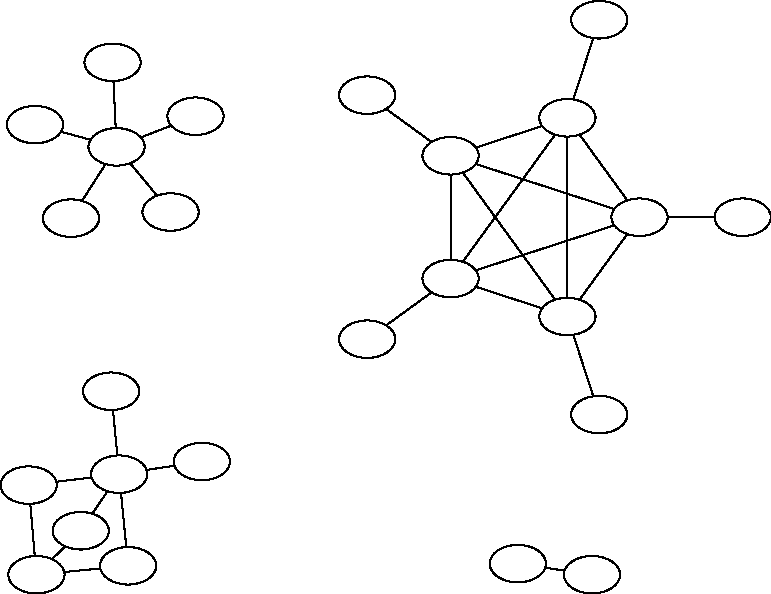
\includegraphics[width=0.9\textwidth]{images/ec2_example.pdf}}

\caption[Chlpaté $2$-hranovo súvislé grafy]{Ukážka štyroch
chlpatých $2$-hranovo súvislých grafov.}

\label{graf:ec2}
\end{figure}

Trieda grafov, ktoré nevieme podľa predošlého dôsledku rozdeliť, obsahuje aj grafy,
v ktorých každý most spája jediný vrchol so zvyškom grafu. Niekoľko takýchto grafov je
znázornených na obrázku \ref{graf:ec2}.

\begin{defn}
    Graf $G$ budeme nazývať \emph{chlpatý $2$-hranovo súvislý graf}, ak je súvislý a pre
    každú mostovú hranu $e \in E(G)$ platí, že jeden z komponentov súvislosti grafu
    $G - \{e\}$ obsahuje jeden vrchol.
\end{defn}

Pripomeňme si, že každý graf, bez ohľadu na jeho štruktúru, má triviálne $L(2,1)$-farbenie
s rozsahom $2n - 2$, kde každému vrcholu priradíme rôzne párne číslo. Pokiaľ pri rozdelení
grafu na dva komponenty ostane jeden z nich dostatočne malý v porovnaní s hodnotou $k$,
pre každé ohodnotenie mostových vrcholov vieme nájsť jeho triviálne $L(2,1)$-farbenie s
rozsahom $k$. Tento fakt zachytáva nasledujúce tvrdenie.

\begin{lema}
    Nech $e$ je mostová hrana grafu $G$, nech $u_1, u_2$ sú vrcholy incidentné s $e$,
    nech $G_1, G_2$ sú komponenty grafu $G - e$, nech vrchol $u_1$ leží v komponente $G_1$ a vrchol $u_2$
    v komponente $G_2$ a
    nech $n_1$ je počet vrcholov komponentu $G_1$. Ak $2n_1 \leq k$, tak $k$-$L(2,1)$-farbenie
    grafu $G$ existuje práve vtedy, ak existuje $k$-$L(2,1)$-farbenie grafu $G_2 \cup \{e, u_1\}$.
\end{lema}

\begin{proof}
    Implikácia $\boxed{\Rightarrow}$ triviálne platí, dokazovať budeme iba $\boxed{\Leftarrow}$.

    Ukážeme, že ľubovoľné $k$-$L(2,1)$-farbenie $f$ grafu $G_2 \cup \{e, u_1\}$ vieme doplniť na
    $k$-$L(2,1)$-farbenie grafu $G$ s tým, že použijeme iba hodnoty z množiny $\{0, 1, \ldots, 2n_1\}$.
    Presnejšie, dokážeme existenciu množiny farieb $F$ obsahujúcu $f(u_1)$, neobsahujúcu $f(u_2)$,
    v ktorej rozdiel každej dvojice prvkov bude aspoň $2$ a ktorej veľkosť bude aspoň $n_1$.
    
    Graf $G_1$ má $n_1$ vrcholov, vrchol $u_1$ z neho už má priradenú niektorú farbu z $F$. Keď vrcholom
    grafu $G_1 - \{u_1\}$ ľubovoľne priradíme rôzne hodnoty z $F - \{f(u_1)\}$, dostaneme $k$-$L(2,1)$-farbenie
    grafu $G$.

    Rozoberieme niekoľko prípadov:

    \begin{description}
        \item[$\boxed{f(u_1) \not\equiv f(u_2) \pmod{2}}:$] 
            Ak je $f(u_1)$ párne, vezmeme $F = \{0, 2, 4, \ldots, 2n_1\}$.
            Ak je $f(u_1)$ nepárne, vezmeme $F = \{1, 3, 5, \ldots, 2n_1 - 1\}$. V oboch prípadoch majú všetky
            čísla v $F$ inú paritu, ako $f(u_2)$, čiže $f(u_2) \notin F$. Zároveň je veľkosť $F$ aspoň $n_1$.

        \item[$\boxed{f(u_1) \equiv f(u_2) \pmod{2} \wedge f(u_1) < f(u_2)}:$]
            Ak je $f(u_2)$ párne, použijeme množinu
            $F = \{0, 2, \ldots, f(u_1), f(u_1) + 3, f(u_1) + 5, \ldots, 2n_1 - 1\}$. Všetky čísla v $F$, ktoré sú
            väčšie, ako $f(u_2)$, majú inú paritu než $f(u_2)$.

            Podobne pre nepárne $f(u_2)$ použijeme množinu $F = \{1, 3, \ldots, f(u_1), f(u_1) + 3, \\ f(u_1) + 5, \ldots, 2n\}$.

        \item[$\boxed{f(u_1) \equiv f(u_2) \pmod{2} \wedge f(u_1) > f(u_2)}:$]
            Analogicky k predošlému prípadu, pre párne $f(u_2)$ použijeme množinu $F = \{1, 3, \ldots, f(u_1) - 3, f(u_1), f(u_1) + 2, \ldots, 2n_1\}$
            a pre nepárne $f(u_2)$ množinu $\{0, 2, \ldots, f(u_1) - 3, f(u_1), f(u_1) + 2, \ldots, 2n_1 - 1\}$. \qedhere
    \end{description}
\end{proof}

Pokiaľ overujeme existenciu $L(2,1)$-farbenia s rozsahom $k$ pre dostatočne veľké $k$ a v grafe
nájdeme most, ktorého odstránením bude prvý komponent malý a druhý veľký, podľa tejto lemy
môžeme malý komponent odignorovať.

Keď v grafe objavíme most, ktorý delí graf na dve podobne veľké časti, môžeme si dovoliť
obe vyriešiť pomocou algoritmu Junosza-Szaniawski. Najväčší problém teda budú spôsobovať
grafy, v ktorých bude veľa mostov oddeľovať stredne veľké podgrafy od zvyšku.

\subsection{Pseudoblokovo-mostový strom}

Pri skúmaní grafov vzhľadom na bloky sa uplatnil pojem blokovo-artikulačného stromu.
Podobný pojem vzhľadom na chlpaté $2$-hranovo súvislé grafy nám pomôže pri konštrukcii
algoritmu a zdôvodnení jeho zložitosti.

\begin{defn}
    Nech $G$ je súvislý graf, nech $E$ je množina všetkých netriviálnych mostov v $G$, nech
    $K_1, K_2 \ldots K_m$ sú komponenty súvislosti grafu $G - E$. Pod pojmom \emph{pseudoblokovo-mostový
    strom grafu $G$} budeme rozumieť graf s ohodnotenými vrholmi $v_1, v_2, \ldots, v_m$, kde
    vrchol $v_i$ má priradenú hodnotu $|V(K_i)|$ a vrcholy $v_i$ a $v_j$ sú spojené hranou
    práve vtedy, keď existuje hrana $e \in E$, ktorá prepája nejaký vrchol v komponente $K_i$
    s nejakým vrcholom v komponente $K_j$.
\end{defn}

Z daného grafu $G$ s $n$ vrcholmi a $m$ hranami vieme zostrojiť jeho pseudoblokovo-mostový graf 
v čase $O(n+m) = O(n^2)$. Pre všetky hrany grafu zistíme, či sú mostové pomocou Tarjanovho
algoritmu \cite{tarjan_bridge}. Pre ľubovoľný most $e$ vieme v konštantnom čase overiť, či je
netriviálny: Pre oba koncové vrcholy $e$ skontrolujeme, či sú incidentné aj s inou hranou, ako $e$.
Keď poznáme netriviálne mosty, vhodným prehľadaním grafu, ktoré nebude môcť prejsť cez netriviálny most,
vieme zistiť aj ohodnotenie vrcholov v pseudoblokovo-mostovom grafe v čase $O(n+m)$.

Medzi všeobecne známe vlastnosti stromov patrí aj existencia vyváženého vrcholového separátora:
V každom strome $T$ existuje vrchol $v$ taký, že každý komponent grafu $T-v$ má nanajvýš polovicu
vrcholov z $T$. Podobné tvrdenie platí aj pre ohodnotené stromy:

\begin{lema}
    \label{stromsep_lema}
    Nech $T$ je $n$-vrcholový strom s kladným ohodnotením vrcholov, nech $s$ je súčet hodnotení jeho vrcholov.
    Potom existuje vrchol $v \in V(T)$ taký, že súčet hodnotení vrcholov v každom komponente
    grafu $T - v$ je nanajvýš $\frac{s}{2}$.
\end{lema}
\begin{proof}
    Dôkaz sporom. Pre každý vrchol $v \in V(T)$ existuje komponent grafu $T - v$, ktorý
    má súčet ohodnotení viac ako $\frac{s}{2}$. Pre každý vrchol môže byť takýto komponent nanajvýš
    jeden, lebo dva komponenty so súčtom hodnotení viac ako $\frac{s}{2}$ sú v spore so súčtom
    hodnotení v $T$.

    Pre každý vrchol $v$ teda existuje práve jeden komponent $K$ súvislosti grafu
    $T - v$, ktorý má súčet hodnotení viac ako $\frac{s}{2}$. Vrchol $v$ je hranou spojený
    s práve jedným vrcholom v každom komponente $T - v$, čiže je spojený s presne identifikovaným
    vrcholom $u$ v komponente $K$. Na hranu $(uv)$ nakreslíme šípku od $v$ k $u$. Tento postup
    vykonáme pre každý vrchol v grafe $T$, čiže $n$-krát.

    Hrán v $n$-vrcholovom strome je $n-1$, teda aspoň na jednu hranu sme nakreslili dve šípky.
    Nech táto hrana spája vrcholy $u$ a $v$. Komponent grafu $T - u$, ktorý obsahuje vrchol $v$,
    označíme $K_v$ a podobne komponent grafu $T - v$ obsahujúci vrchol $u$ označíme $K_v$. Kedže
    hrana $(uv)$ dostala dve šípky, komponenty $K_u$ aj $K_v$ musia mať súčet ohodnotení viac ako
    $\frac{s}{2}$. Komponenty $K_u$ a $K_v$ však majú disjunktné množiny vrcholov, čo je v spore
    s faktom, že súčet hodnotení vrcholov v $T$ je $s$. \qedhere
\end{proof}

Z dôkazu predošlej lemy nám taktiež vyplýva algoritmus, ktorým vieme v polynomiálnom čase
nájsť takýto vrchol $v$. Najprv v čase $O(n)$ spočítame súčet hodnotení vrcholov. Potom začneme
v nejakom vrchole $u$, spočítame súčet hodnotení v každom komponente grafu $G - u$ (v lineárnom čase).
Ak má niektorý komponent priveľký súčet, nájdeme v ňom vrchol, ktorý susedí s $u$ a proces opakujeme.
V opačnom prípade sme našli vrchol $v$ spĺňajúci lemu.

Pri tomto procese nemôžeme navštíviť žiaden vrchol viackrát, ináč by sme dostali buď spor s
acyklickosťou stromu $T$, alebo by sme dostali podobný spor, ako na konci dôkazu. Algoritmus
na hľadanie vrcholu $v$ sa dá dokonca spraviť v lineárnom čase od počtu vrcholov $T$, ale nám
stačí ľubovoľný polynomiálny čas.

Nakoniec budeme potrebovať ešte dva stavebné algoritmy k našej redukcii. Jedným z nich je
viackrát spomínaný algoritmus Junosza-Szaniawski, ktorý vie riešiť problém doplnenia $L(2,1)$-farbenia
v ľubovoľnom súvislom grafe v čase $O^*(2.6488^n)$ \cite{junosza_fast}. Druhým z nich je algoritmus od Haveta
a kol., ktorý vie riešiť problém $L(2,1)$-farbenia pre rozsah $k \leq 5$ v čase $O^*(2.5^n)$ \cite{havet}.

\subsection{Algoritmus na rozdelenie problému}

Nakoniec ukážeme, ako môžeme ľubovoľný algoritmus $\mathcal{B}$, ktorý rieši problém doplnenia
$L(2,1)$-farbenia na chlpatých $2$-hranovo súvislých grafoch, prerobiť na algoritmus $\mathcal{A}$, ktorý
rieši problém $L(2,1)$-farbenia na všeobecných grafoch. Ak je časová zložitosť $\mathcal{B}$
$O^*(\alpha^n)$ pre nejaké $\alpha \ge 2.55$, bude časová zložitosť algoritmu $\mathcal{A}$ tiež
$O^*(\alpha^n)$.

Algoritmus $\mathcal{A}$ dostane na vstupe súvislý graf $G$ a číslo $k$ a akceptuje práve vtedy,
keď existuje $L(2,1)$-farbenie grafu $G$ s rozsahom $k$. Popis algoritmu:

\begin{enumerate}
    \item Ak $k \ge 2n$, akceptuj. $O^*(1)$
    \item Ak $k \leq 5$, spusti a vráť výsledok algoritmu od Haveta a kol. $O^*(2.5^n)$
    \item Nájdi všetky netriviálne mosty grafu $G$. $O^*(1)$
    \item Ak $G$ nemá netriviálne mosty, spusti a vráť výsledok algoritmu $\mathcal{B}$. $O^*(\alpha^n)$
    \item Vytvor pseudoblokovo-mostový strom $T$ grafu $G$. $O^*(1)$
    \item Kým $T$ obsahuje listový vrchol $l$ s hodnotou nanajvýš $\frac{k}{2}$, odstráň
          z $T$ vrchol $l$ a zvýš rodičovi $l$ hodnotu o $1$. V grafe $G$ odstráň podgraf
          zodpovedajúci vrcholu $l$ okrem hrany a vrcholu, ktorý ho pripájajú ku zvyšku grafu. $O^*(1)$
    \item Ak je $G$ po predošlom kroku chlpatý $2$-hranovo súvislý graf, spusti algoritmus $\mathcal{B}$. $O^*(\alpha^n)$
    \item Nájdi vrchol $v$ grafu $T$, ktorý
          spĺňa lemu o rovnovážnom rozdelení stromu \ref{stromsep-lema}. $O^*(1)$
    \item Pre každý komponent $K_i$ grafu $T - v$ spočítaj súčet jeho hodnôt $s_i$. $O^*(1)$
    \item Ak pre niektorý komponent $K_i$ je hodnota $s_i$ väčšia ako $\frac{n}{10}$,
          nájdi hranu $e'$, ktorá pripája $K_i$ k $v$ v grafe $T$ a zodpovedajúci most
          $e = (uw)$ v grafe $G$. Pre každé ohodnotenie vrcholov $u, w$ spusti upravený
          algoritmus Junosza-Szaniawski na komponentoch grafu $G - e$. Akceptuj, ak pre
          niektoré ohodnotenie vrcholov $u, w$ algoritmus Junosza-Szaniawski akceptoval
          na oboch komponentoch grafu $G-e$ zároveň. V opačnom prípade zamietni. $O^*(2.6488^{\frac{9n}{10}})$
    \item Nájdi všetky hrany $e_i$ v grafe $G$, ktoré zodpovedajú hranám v $T$ incidentným s
          vrcholom $v$. Vyskúšaj všetky možné priradenia hodnôt vrcholom incidentným s
          niektorou hranou $e_i$. Pre každé priradenie hodnôt spusti algoritmus $\mathcal{B}$ na podgrafe
          v $G$ zodpovedajúcemu vrcholu $v$ v $T$ a prispôsobený algoritmus Junosza-Szaniawski na podgrafoch
          $G$, ktoré zodpovedajú komponentom grafu $T - v$.
\end{enumerate}

======================= Pod tymto vsetko zmazat? ============================================

Pokiaľ overujeme existenciu $k$-$L(2,1)$-farbenia pre dostatočne veľkú hodnotu $k$ a v grafe
nájdeme most, ktorého odstránením bude prvý komponent malý a druhý veľký, podľa tejto lemy
môžeme malý komponent odignorovať. Pri takomto prístupe by nám mohli robiť problém malé
hodnoty $k$. Tie môžeme vyriešiť s použitím algoritmu od Haveta a kol., ktorý rieši
problém $L(2,1)$-farbenia pre $k \leq 5$ v čase $O^*(2.5^n)$ \cite{havet}. Tento
algoritmus principiálne prehľadáva všetky $k$-$L(2,1)$-farbenia grafu, preto sa dá
priamočiaro prerobiť na algoritmus, ktorý rieši problém doplnenia $L(2,1)$-farbenia.

Teraz máme všetky podklady pre to, aby sme vedeli upraviť algoritmus,
ktorý rieši problém doplnenia $L(2,1)$-farbenia na chlpatých
$2$-hranovo súvislých grafoch, na algoritmus riešiaci problém $L(2,1)$-farbenia
na súvislých grafoch. Do pozornosti dávame, že náš algoritmus nebude riešiť
problém doplnenia $L(2,1)$-farbenia.

\begin{veta}
    FIXME: Toto v skutocnosti nefunguje. Rozbit na viacero pripadov, tato veta moze pokryvat pripad, ze
    pseudobloky su dostatocne velke. Doriesit pripady, kedy mozu byt pseudobloky male.

    Ak existuje algoritmus $\mathcal{B}$, ktorý rieši rozhodovací problém zoznamového $L(2,1)$-farbenia
    na chlpatých $2$-hranovo-súvislých grafoch s časovou zložitosťou $O^*(\alpha^n)$, kde
    $\alpha \ge 2.5$, tak existuje algoritmus $\mathcal{A}$, ktorý rieši problém $L(2,1)$-farbenia
    na súvislých grafoch s časovou zložitosťou $O^*(\alpha^n)$.
\end{veta}

\begin{proof}
    Najprv skonštruujeme algoritmus $\mathcal{A}$, ktorý dostane hodnotu $k$, graf $G$ a zoznam
    povolených hodnôt $c$. Algoritmus bude fungovať nasledovne:

    \begin{enumerate}
        \item Ak $k \leq 5$, spusti algoritmus od Haveta a kol.
        \item Ak $G$ je chlpatý $2$-hranovo-súvislý graf, spusti a vráť výstup algoritmu $\mathcal{B}$.
        \item Inak sa v grafe nachádza netriviálny most. Nájdi most $e$ s koncovými vrcholmi $u, v$.
        Skonštruuj graf $G_1$ ako komponent súvislosti grafu $G - \{e\}$ obsahujúci $u$ a $G_2$ ako
        komponent súvislosti obsahujúci $v$. Bez ujmy na všeobecnosti platí $|V(G_1)| \leq |V(G_2)|$.
        V prípade viacerých možností pre výber mostu $e$ vyber niektorý z tých, pre ktoré je počet
        vrcholov v grafe $G_1$ najmenší.
        \item Ak $\left |V(G_1) \right| \leq \frac{k}{2}$, rekurzívne spusti a vráť výstup algoritmu
        $\mathcal{A}$ na grafe $G_2 \cup \{e, u\}$ s príslušne zúženým zoznamom hodnôt $c$.
        \item Pre všetky prípustné (podľa $c$) ofarbenia $f$ vrcholov $u, v$ spusti rekurzívne
        algoritmus $\mathcal{A}$ na grafe $G_1 \cup \{e, v\}$. V každom volaní je zoznam $c$ zúžený
        na príslušnú množinu vrcholov a navyše $c(u) = \{f(u)\}$ a $c(v) = \{f(v)\}$. Zoznam dvojíc
        $(f(u), f(v))$, pre ktoré výpočet akceptoval, označíme $Z$.
        \item Pre všetky prípustné (podľa $c$) ofarbenia $f(u)$ vrchola $u$ spusti rekurzívne
        algoritmus $\mathcal{A}$ na grafe $G_2 \cup \{e, u\}$. V každom volaní je zoznam $c$ zúžený
        na príslušnú množinu vrcholov a navyše $c(u) = \{f(u)\}$ a $c(v) = \{x | (f(u), x) \in Z\}$.
        \item Ak aspoň jedno z rekurzívnych volaní v 6. kroku akceptovalo, akceptuj. V opačnom prípade
        zamietni.
    \end{enumerate}

    Overenie, či graf patrí do triedy chlpatých $2$-hranovo-súvislých grafov, vieme realizovať v čase
    $O(|V(G)| + |E(G)|)$ nájdením všetkých mostov pomocou Tarjanovho
    algoritmu \cite{tarjan_bridge}. Prehľadávaním do hĺbky vieme v čase $O(|V(G)| + |E(G)|)$ pre
    každý most a pre každý komponent, ktorý jeho odstránenie indukuje, spočítať, koľko vrcholov obsahuje.
    Zvyšné manipulácie s dátami vieme pri vhodnej reprezentácii robiť v polynomiálnom čase.

    Pokiaľ platí podmienka v kroku 1, alebo v kroku 2, časová zložitosť algoritmu je nanajvýš
    $T(n) \leq O^*(1) + O^*(\alpha^n)$.

    Pokiaľ sa vykoná krok 4, graf $G_2$ bude obsahovať nanajvýš $n-1$ vrcholov, z čoho dostávame
    vzťah pre časovú zložitosť $T(n) \leq O^*(1) + T(n-1)$.

    Pre hodnotu $k \ge 6$ spočítame, koľkými spôsobmi môžeme ofarbiť dvojicu susedných vrcholov $u, v$.
    Pokiaľ vrchol $u$ ofarbíme farbou $x$, vrchol $v$ môže dostať ľubovoľnú farbu okrem $x, x-1$ a $x + 1$.
    To znamená, že ak vrchol $u$ ofarbíme farbou $0$ alebo $k$, ostane nám pre vrchol $k + 1 - 2$ možností.
    Ak vrchol $u$ ofarbíme ktoroukoľvek zo zvyšných $k-1$ možností, pre vrchol $v$ nám vždy ostane $k + 1 - 3$
    možností. Úpravou dostaneme, že počet ofarbení týchto vrcholov je $2(k-1) + (k-1)(k-2) = k(k-1)$.

    Ďalej označíme $n_1$ ako počet vrcholov komponentu $G_1$. 
    Krok 5 zahŕňa $k(k-1)$ spustení algoritmu na grafe $G_1 \cup \{e, v\}$, ktorý má $n_1 + 1$
    vrcholov. Krok 6 zahŕňa nanajvýš $k+1$ spustení algoritmu na grafe $G_2 \cup \{e, u\}$, ktorý
    má $n - n_1 + 1$ vrcholov. Časová zložitosť tejto vetvy výpočtu teda spĺňa vzťah 
    $$T(n) \leq O^*(1) + k(k-1)T(n_1+1) + (k+1)T(n - n_1 + 1).$$

    Ďalej dokážeme, že pre vhodne zvolený polynóm $q$ je časová zložitosť
    algoritmu $\mathcal{A}$ nanajvýš $q(n) \alpha^n$.

    Nech $p$ je neklesajúci polynóm, pre ktorý platí, že časová zložitosť algoritmu $\mathcal{B}$ aj algoritmu
    od Haveta a kol. je zhora ohraničená $p(n)\alpha^n$. Nech $s$ je neklesajúci polynóm, ktorý
    zhora ohraničuje časovú zložitosť jedného volania algoritmu $\mathcal{A}$, bez započítania 
    rekurzívnych volaní a volaní iných algoritmov. Nech $r$ je neklesajúci polynóm, ktorý spĺňa
    $\forall n \in \mathbb{N}: r(n) \ge p(n)$ a navyše pre $n \leq 20$ je hodnota $r(n)$ horným
    ohraničením na časovú zložitosť algoritmu $\mathcal{A}$ na grafe s $n$ vrcholmi.

    Nakoniec polynóm $q$ určíme vzťahom $q(n) = r(n) + n \cdot s(n)$. Za zmienku stojí, že takto
    definovaný polynóm $q$ je tiež neklesajúci. Ďalej matematickou indukciou
    dokážeme, že časová zložitosť algoritmu $\mathcal{A}$ na grafe s $n$ vrcholmi je zhora ohraničená
    funkciou $q(n) \alpha^n$. Bázou indukcie bude tvrdenie, že pre $n \leq 20$ ohraničenie platí. Toto
    triviálne vyplýva z definície polynómov $r(n)$ a $q(n)$. Pre dôkaz indukčného kroku rozoberieme
    všetky možnosti vetvenia algoritmu $\mathcal{A}$.

    Pokiaľ platí podmienka v 1. alebo 2. kroku,
    $q(n) \alpha^n \ge p(n) \alpha^n + s(n)$ vyplýva z nerovností $q(n) \ge r(n) + s(n) \ge p(n) + s(n)$.

    Pokiaľ platí podmienka v 4. kroku, potrebujeme dokázať $q(n) \alpha^n \ge q(n-1) \alpha^{n-1} + s(n)$:
    $$ q(n) \alpha^n \ge q(n) \alpha^{n-1} = \left(r(n) + n \cdot s(n) \right) \alpha^{n-1} \ge s(n) + \left(r(n) + (n-1)s(n) \right) \alpha^{n-1} \ge $$
    $$ \ge s(n) + \left(r(n-1) + (n-1)s(n-1) \right) \alpha^{n-1} = s(n) + q(n-1) \alpha^{n-1}$$.

    Pokiaľ sa vykoná 5. a 6. krok, potrebujeme dokázať

    $$q(n) \alpha^n \ge k(k-1)q(n_1+1)\alpha^{n_1 + 1} + (k+1)q(n - n_1 + 1)\alpha^{n - n_1 + 1} + s(n).$$

    Kvôli prehľadnosti zasubstituujeme členy v predošlej nerovnosti: $a := q(n) \alpha^n,\\ b :=  k(k-1)q(n_1+1)\alpha^{n_1 + 1},
    c := (k+1)q(n - n_1 + 1)\alpha^{n - n_1 + 1}, d := s(n)$. Potrebujeme dokázať $a \ge b + c + d$.
    Rozoberieme zopár prípadov. Ak $c \ge b + d$, stačí dokázať $a \ge 2c$. Inak platí $c < b + d$ a
    teda stačí dokázať $a \ge 2(b + d)$. Opäť rozoberieme prípady podľa veľkosti výrazov. Ak $b \ge 2d$,
    stačí dokázať $a \ge 3b$, v opačnom prípade stačí dokázať $a \ge 6d$. Ak teda platí
    $a \ge 2c \wedge a \ge 3b \wedge a \ge 6d$, zaručene platí aj $a \ge b + c + d$. Všetky
    tri prípady rozoberieme:

    \begin{description}
    \item[$\boxed{a \ge 6d}$], čiže $q(n) \alpha^n \ge 6s(n)$. Keďže indukčný
    krok dokazujeme pre $n \ge 20$, platí $q(n) \alpha^n \ge q(n) = r(n) + n\cdot s(n) \ge
    20s(n) \ge 6s(n)$.

    \item[$\boxed{a \ge 3b}$], čiže $q(n) \alpha^n \ge 3k(k-1)q(n_1 + 1)\alpha^{n_1 + 1}$.
    Z algoritmu máme predpoklad, že komponent $G_1$ má nanajvýš toľko vrcholov, čo $G_2$, preto
    $n_1 \leq \frac{n}{2}$. Z neklesajúcosti $q$ a exponenciálnej funkcie platí $q(n_1 + 1)\alpha^{n_1 + 1}
    \leq q(n) \alpha^{\frac{n}{2} + 1}$. Nakoniec využijeme nerovnosť $k < 2n_1 \leq n$, ktorá musí platiť,
    aby algoritmus $\mathcal{A}$ neskončil už v kroku 4.

    $$3k(k-1)q(n_1 + 1)\alpha^{n_1 + 1} \leq 3k(k-1)q(n)\alpha^{\frac{n}{2} + 1} = \frac{3k(k-1)}{\alpha^{\frac{n}{2} - 1}}q(n)\alpha^n < \frac{3n(n-1)}{\alpha^{\frac{n}{2} - 1}}q(n)\alpha^n$$

    Nakoniec potrebujeme dokázať $\frac{3n(n-1)}{\alpha^{\frac{n}{2}-1}} \leq 1$. Pre $n > 20$ je čitateľ aj
    menovateľ kladný, preto stačí dokázať $3n(n-1) \leq \alpha^{\frac{n}{2} - 1}$. Keďže $\alpha \ge 2.5$,
    stačí nám dokázať $3n(n-1) \leq 2.5^{\frac{n}{2} - 1}$. Pre $n = 20$ táto nerovnosť platí a navyše
    pre $n \ge 20$ je derivácia funkcie na ľavej strane menšia, ako derivácia funkcie na pravej strane.
    Z toho vyplýva nerovnosť $3n(n-1) \leq 2.5^{\frac{n}{2}-1}$ a aj dokazovaná nerovnosť.

    \item[$\boxed{a \ge 2c}$], čiže $q(n) \alpha^n \ge 2(k+1)q(n - n_1 + 1)\alpha^{n - n_1 + 1}$.
    Opäť využijeme fakt, že $k < 2n_1$. Z netriviálnosti komponentu $G_1$ vyplýva $n - n_1 + 1 < n$ 

    $$2(k+1)q(n - n_1 + 1)\alpha^{n - n_1 + 1} \leq \frac{2(k+1)}{\alpha^{n_1 - 1}}q(n)\alpha^n < \frac{2k + 2}{\alpha^{\frac{k}{2} - 1}} q(n)\alpha^n$$

    Aby platila nerovnosť, stačí teda dokázať $\frac{2k + 2}{\alpha^{\frac{k}{2} - 1}} \leq 1$. Keďže
    $f(k) = 2k + 2$ aj $g(k) = \alpha^{\frac{k}{2} - 1}$ sú pre $k \ge 6$ kladné, stačí dokázať
    $f(k) \leq g(k)$. Pre $k = 9$ nerovnosť platí a pre $k \ge 9$ platí $f'(x) \leq g'(x)$.

    Pre $k \ge 9$ teda nerovnosť platí. Pre $k \in \{6, 7, 8\}$ musíme odhad robiť presnejšie.
    Potrebujeme dobre odhadnúť zlomok $\frac{2k+2}{\alpha^{n_1 - 1}}$. Z nerovnosti $k < 2n_1$
    vyplýva, že pre $k \in \{6, 7\}$ platí $n_1 \ge 4$ a pre $k = 8$ platí $n_1 \ge 5$.

    Pre $k=6$ a $n_1 \ge 4$ je zlomok $\frac{2k+2}{n_1 - 1}$ zhora ohraničený hodnotou $\frac{14}{2.5^3} \leq 0.9$,
    pre $k=8$ a $n_1 \ge 5$ je zlomok $\frac{2k+2}{n_1 - 1}$ zhora ohraničený hodnotou $\frac{18}{2.5^4} \leq 0.5$.

    Pre $k=7$ potrebujeme odhad s $n_1 \ge 4$. Pre $n_1 = 4$ má ale zlomok $\frac{2k+2}{n_1 - 1}$ hodnotu
    väčšiu ako $1$. Pre $n_1 \ge 5$ je zlomok $\frac{16}{2.5^{n_1}}$ zhora ohraničený hodnotou $\frac{16}{2.5^4} \leq 0.5$.

    Pre všetky hodnoty $k \ge 6$ a $n_1 \ge \frac{k}{2}$ okrem dvojice $(7, 4)$ teda platí
    $$q^n \alpha^n \ge 2(k+1)\alpha^{n - n_1 + 1}.$$

    \end{description}

    Pre takmer všetky možnosti $k$ a $n_1$, pre ktoré algoritmus $\mathcal{A}$ vykoná kroky 5, 6 a 7,
    sme dokázali, že $q(n) \alpha^n$ je horným odhadom pre jeho časovú zložitosť. Jediná kombinácia
    $k$ a $n_1$, pre ktorú sme to zatiaľ nedokázali, je $k=7$ a $n_1 = 4$. Špeciálne pre tieto hodnoty
    spravíme presnejší odhad.

    Potrebujeme teda dokázať $q(n) \alpha^n \ge 42 \cdot q(5) \alpha^5 + 8 \cdot q(n - 3) \alpha^{n-3} + s(n)$.
    Keďže dokazujeme indukčný krok, môžeme predpokladať $n \ge 20$.

    $$q(n) \alpha^n = \left(r(n) + n \cdot s(n) \right) \alpha^n \ge \left(r(n) + (n-1)s(n) \right) \alpha^n + s(n) \ge q(n-3) \alpha^n + s(n) \ge$$
    $$\ge \left(\frac{2.5}{2} \right)^3 \cdot 8 \cdot q(n-3) \alpha^{n-3} + s(n) = \left( \frac{61}{64} + 1\right) \cdot 8 \cdot q(n-3)\alpha^{n-3} + s(n) \ge $$
    $$\ge q(n-3) \alpha^{n-3} + 8 \cdot q(n-3) + s(n) \ge^{(*)} q(17) \alpha^{17} + 8 \cdot q(n-3)\alpha^{n-3} + s(n) \ge $$
    $$\ge q(5)2^{12}\alpha^{5} + 8 \cdot q(n-3) + s(n) \ge 42 q(5)\alpha^5 + 8 \cdot q(n-3) + s(n)$$

    Označená nerovnosť platí kvôli $n \ge 20$.

    Týmto sme dokázali, že existuje polynóm $q(n)$ taký, že časová zložitosť algoritmu $\mathcal{A}$ je
    zhora ohraničená funkciou $q(n)\alpha^n$. Preto časová zložitosť algoritmu je $O^*(\alpha^n)$. \qedhere

\end{proof}

Naším cieľom je vytvoriť rýchly algoritmus na riešenie problému $L(2,1)$-farbenia. Posledná veta
nám hovorí, že nám stačí vyriešiť tento problém na chlpatých $2$-hranovo súvislých grafoch. V dôkaze
máme aj návod, ako takéto špecifické riešenie prerobiť na algoritmus na všeobecných grafoch.


